\chapter{Metodologia}
\label{cap:metodologia}

O presente trabalho adota a metodologia \gls{dsr}, conforme descrita por \cite{peffers2007design}, que propõe um modelo estruturado para a construção e avaliação de artefatos tecnológicos. A \gls{dsr} é amplamente utilizada em pesquisas de computação e engenharia de software, pois permite a criação de soluções inovadoras baseadas em problemas reais \citep{horita2019design}.

\section{Fases da Design Science Research}

\cite{peffers2007design} definem seis fases principais para a DSR:

\begin{enumerate}
    \item \textbf{Identificação do Problema e Motivação}: Definição do problema e justificativa de sua relevância.
    \item \textbf{Definição dos Objetivos da Solução}: Especificação do que a solução deve alcançar.
    \item \textbf{Design e Desenvolvimento}: Construção do artefato proposto dividida em ciclos.
    \item \textbf{Demonstração}: Aplicação da solução em um contexto real.
    \item \textbf{Avaliação}: Verificação da eficácia da solução.
    \item \textbf{Comunicação}: Divulgação dos resultados para a comunidade científica e profissionais da área.
\end{enumerate}

Neste trabalho, as fases da DSR foram adaptadas para um modelo de cinco etapas, de forma a organizar melhor o fluxo do projeto:

\begin{enumerate}
    \item \textbf{Identificação do Problema};
    \item \textbf{Definição dos Objetivos da Solução};
    \item \textbf{Design e Desenvolvimento};
    \item \textbf{Avaliação};
    \item \textbf{Comunicação}.
\end{enumerate}

Essa adaptação mantém a essência da DSR ao abranger a identificação do problema, definição dos objetivos, construção da solução, avaliação e comunicação dos resultados, garantindo uma abordagem estruturada e alinhada aos objetivos do projeto.

\section{Fase 1: Identificação do Problema}\label{definicao_do_problema}
As abordagens tradicionais de divulgação digital, baseadas em imagens estáticas e textos, limitam a interatividade e a imersão necessárias para explorar sítios arqueológicos. Essa falta de recursos modernos reduz o engajamento do público e dificulta a compreensão espacial desses patrimônios.
No caso do patrimônio arqueológico de Formosa, Goiás, o site original no Blogger desempenhou um papel importante na documentação inicial e na democratização do acesso a pesquisas sobre o Bisnau. No entanto, suas limitações técnicas, como baixa usabilidade, identidade visual desatualizada e restrições de personalização, comprometem a experiência do usuário e o alcance do conteúdo.
Para superar essas limitações, propôs-se o desenvolvimento de um Ambiente Virtual 3D, que permitirá uma exploração imersiva dos sítios arqueológicos e poderá ser baixado pelo novo site. A validação da proposta incluiu:

\begin{itemize}
\item \textbf{Visitas de campo}: Coleta de imagens e informações sobre os sítios, observando deteriorações como pichações e erosão.
\item \textbf{Análise Heurística}: Avaliação do site original com base nas 10 heurísticas de Nielsen, identificando falhas críticas como navegação confusa e falta de acessibilidade.
\end{itemize}

\subsection{Visitas de Campo}
As visitas de campo foram realizadas no sítio arqueológico da Lapa da Pedra, localizado na região nordeste de Formosa, Goiás. Conforme descrito no Referencial Teórico (\ref{sec:sitio lapa da pedra}), o sítio abriga 29 grutas, das quais sete contêm registros de arte rupestre. A Gruta IV S. = Gruta XIV M.–-47.302462,-15.493179 foi o foco principal deste trabalho, sendo a maior e a que contém mais desenhos.

Durante as visitas, observou-se que as pinturas estão distribuídas em alturas variáveis, desde 0,40 metros até 7,50 metros, em superfícies lisas, saliências e reentrâncias naturais do calcário. Apesar de sua relevância histórica, foram identificados sinais de deterioração tanto natural quanto antrópica. Entre os danos naturais, destacam-se a descamação da tinta, infiltrações e fissuras nas rochas, conforme discutido na seção sobre ameaças à preservação (\ref{sec:amecas a preservação}).

Quanto à ação humana, notou-se pichações e escritas superpostas às pinturas originais (Figura \ref{fig:degradacao vera}), reflexo da falta de conscientização sobre a importância cultural do sítio. Esses indícios reforçam a necessidade de estratégias de preservação digital e divulgação ampla, como discutido na Introdução.
\begin{figure}[H]
    \centering
    \includegraphics[height=8cm, keepaspectratio]{img/Visitas tecnicas/depredacao vera.JPG}
    \caption{Escritas superpostas à pinturas original. \\ Está escrito "Vera visitou em 28 de 10 de 62". \\
        \textbf{Fonte:} Acervo pessoal do Ramon Almeida, 2024.}
    \label{fig:degradacao vera}
\end{figure}

Além disso, a localização do sítio em uma propriedade privada, a Fazenda Pedra, contribuiu para sua preservação parcial, mas também limita o acesso e a visibilidade do patrimônio para a população local. Essa constatação evidencia a urgência de iniciativas que promovam a democratização do acesso ao patrimônio cultural, alinhadas ao objetivo deste projeto.

\subsection{Análise Heurística do Antigo Site}
A análise heurística foi realizada no site antigo hospedado na plataforma Blogger com o auxílio da ferramenta Heurio, utilizando como referência as 10 heurísticas de usabilidade propostas por Jakob Nielsen (1994). A análise foi feita por quatro avaliadores: Naoki Rafael Miura, Victor Hugo Sales dos Reis, Sara Candido Fernandes e Erik Takeshi Miura, que identificaram problemas de usabilidade e navegabilidade.
A Figura \ref{fig:interface heurio} mostra a interface do Heurio, enquanto as Figuras \ref{fig:comentario heurio} e \ref{fig:fluxo} mostram o fluxo para inserir as observações da análise, que envolve a identificação do problema, a sugestão de melhoria e a indicação de qual heurística o problema está relacionado.
\begin{figure}[H]
    \centering
    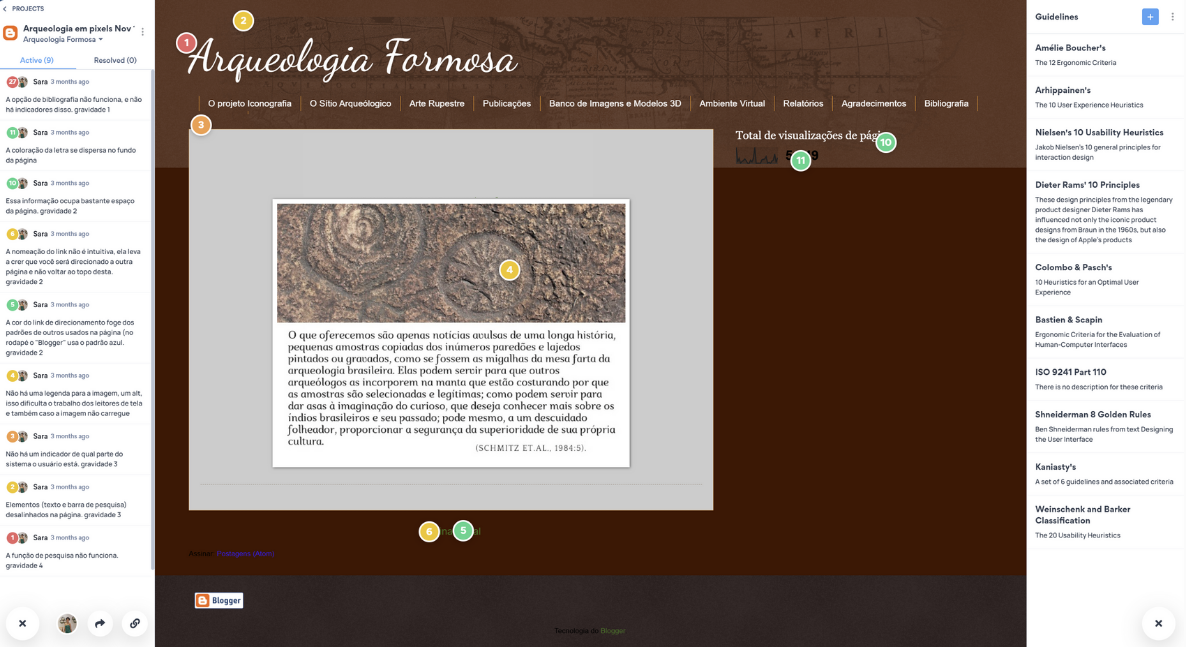
\includegraphics[height=8cm, keepaspectratio]{img/heurio/interface heurio.png}
    \caption{ Interface da ferramenta Heurio. Ela exibe o site a ser analisado, \\ os comentários já feitos no lado esquerdo e os grupos de heurísticas do lado direito. \\
        \textbf{Fonte:} Elaborado pelo autor, 2024.}
    \label{fig:interface heurio}
\end{figure}

\begin{figure}[H]
    \centering
    \begin{minipage}[b]{0.48\textwidth}
        \centering
        \includegraphics[height=6cm, keepaspectratio]{img/heurio/habilitar comentários.png}
        \caption{Botão de habilitar comentários no Heurio.  \\
            \textbf{Fonte:} Elaborado pelo autor, 2024.}
        \label{fig:comentario heurio}
    \end{minipage}
    \hfill
    \begin{minipage}[b]{0.48\textwidth}
        \centering
        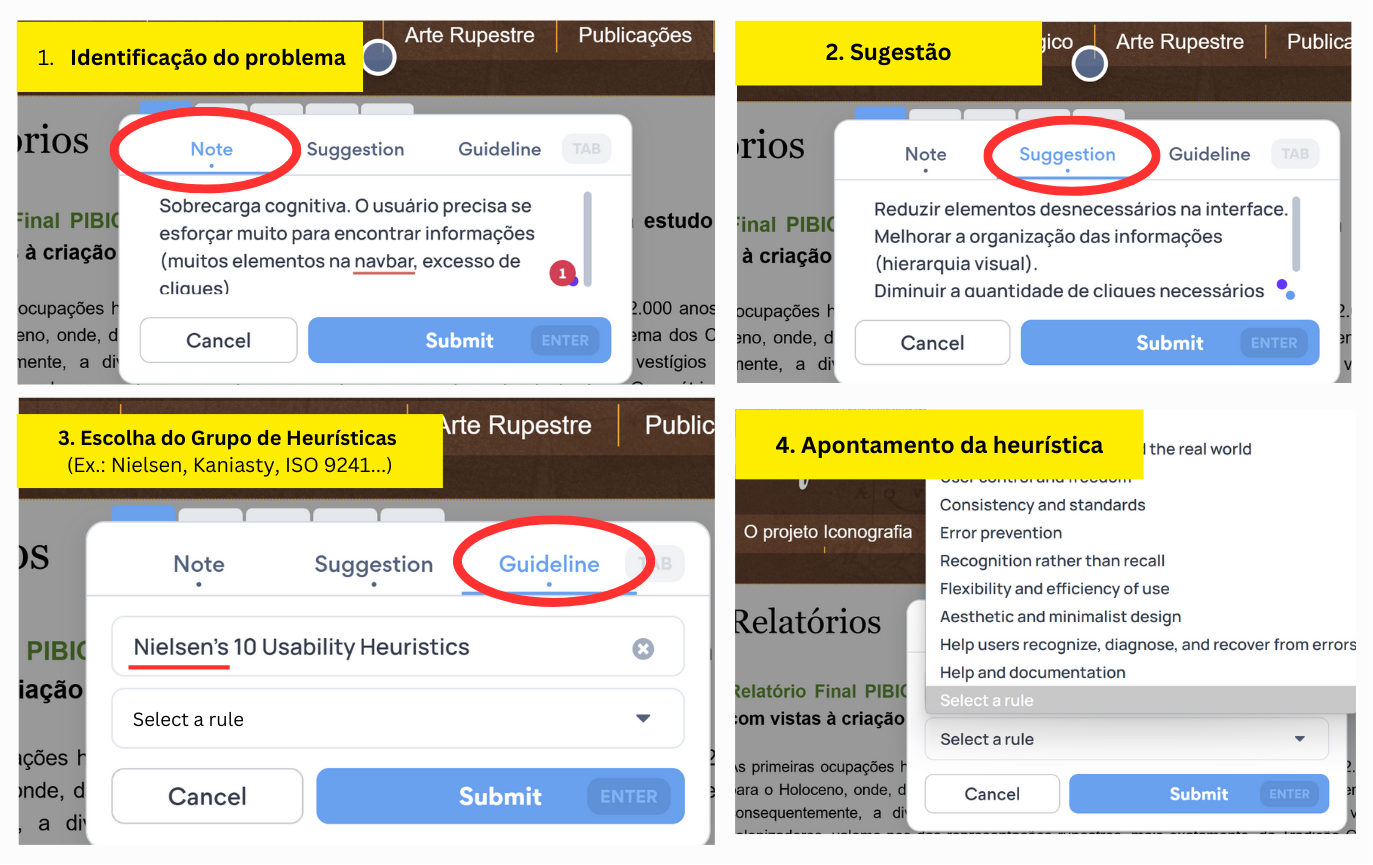
\includegraphics[height=6cm, keepaspectratio]{img/heurio/fluxo heurio.png}
        \caption{Fluxo de observações incluindo identificação \\do problema, sugestão e heurística relacionada. \\
            \textbf{Fonte:} Elaborado pelo autor, 2024.}
        \label{fig:fluxo heurio}
    \end{minipage}
\end{figure}

Por fim, a ferramenta Heurio gera um quadro para visualização como se fosse um relatório (Figura \ref{fig:quadro resultados}). Essas observações de cada um dos analistas foram reunidas e contribuíram para a identificação do problema, possibilitando a melhoria do site. 
\begin{figure}[H]
    \centering
    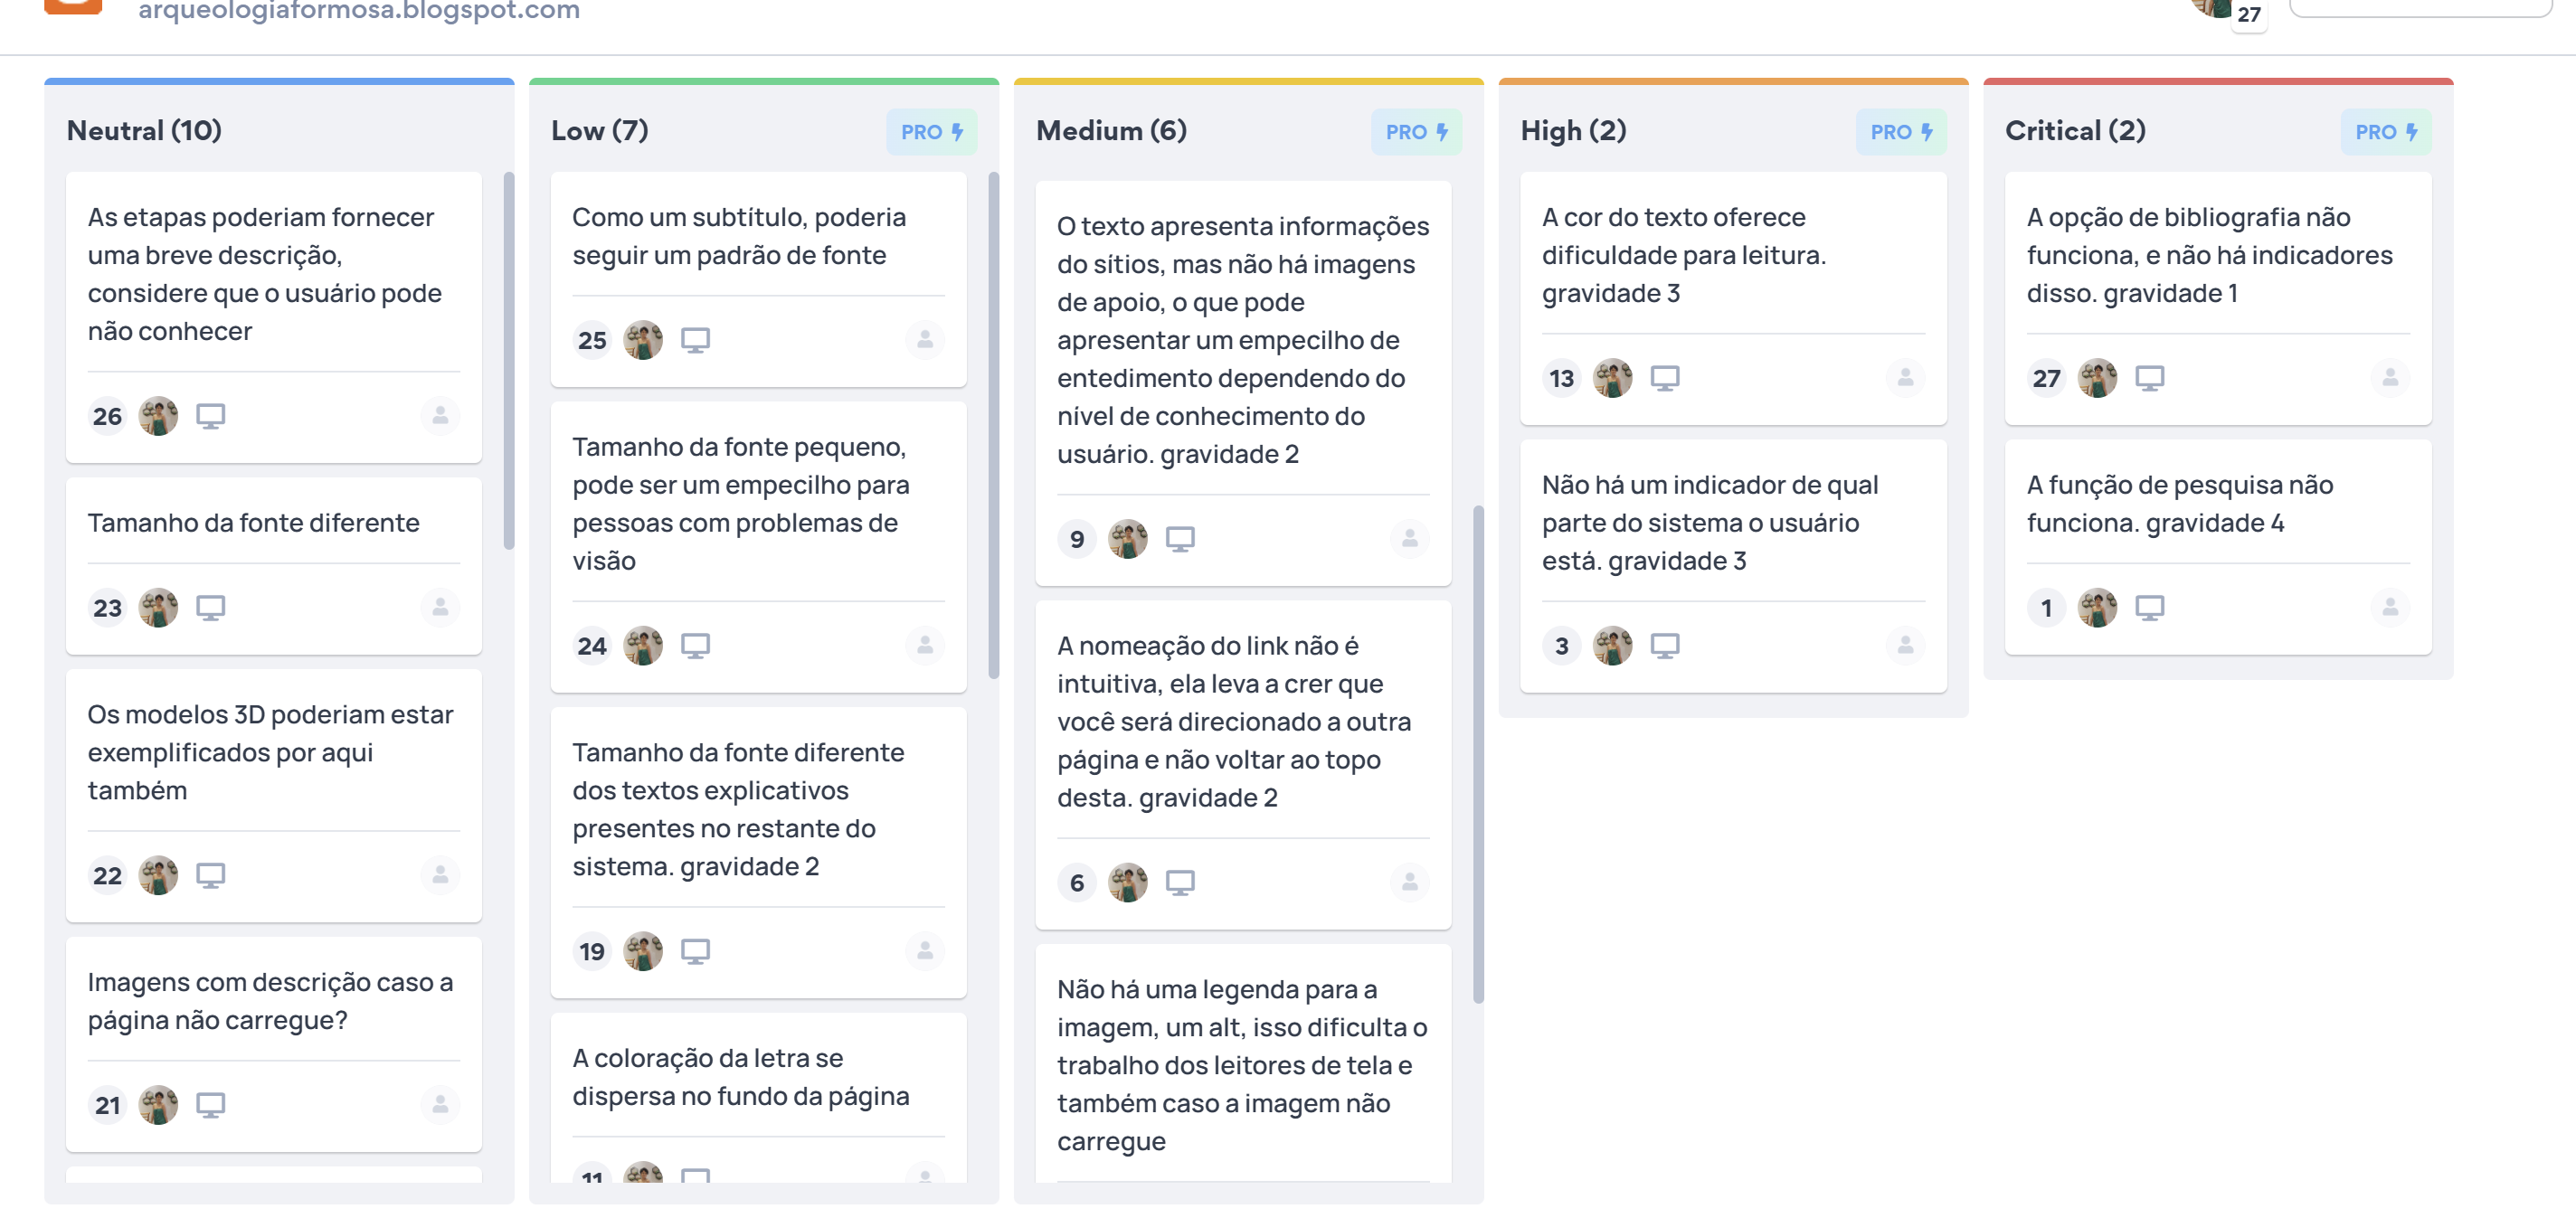
\includegraphics[height=8cm, keepaspectratio]{img/heurio/quadro resultados.png}
    \caption{ Quadro de resultados gerado após a análise do Heurio. \\
        \textbf{Fonte:} Elaborado pelo autor, 2024.}
    \label{fig:quadro resultados}
\end{figure}


\section{Fase 2: Definição dos Objetivos da Solução}\label{definicao_dos_objetivos_da_solucao}
Essa fase envolve a especificação do que a solução deve alcançar. Para isso foi utilizada a técnica de engenharia de requisitos.
\subsection{Coleta de Requisitos}
Coleta de requisitos foi realizada por meio de questionário online e entrevistas formais e informais com professores do IFG, resultando em 13 requisitos funcionais (Apêndice \ref{ap:requisitos-site-table}) e 13 não funcionais (Apêndice \ref{ap:requisitos-nao-funcionais-site-table}) para o site. Para o ambiente virtual há quatro requisitos funcionais (Apêndice \ref{ap:requisitos-ambiente-table}) e 2 requisitos não funcionais (Apêndice \ref{ap:requisitos-nao-funcionais-ambiente}). Todos os requisitos podem ser consultados no apêndice. 

\subsubsection{Identificação dos Requisitos}
\label{sec:identificacao_requisitos}

Por convenção e para facilitar a identificação dos casos de uso junto aos contextos, a referência é feita de acordo com o esquema abaixo:

\textbf{Sigla de subseção | numeração}

Os requisitos são identificados por uma sigla que representa a subseção (por exemplo, "RFS" para Requisitos Funcionais do site, “RNFA” para Requisitos Não Funcionais do Ambiente Virtual) seguida de um número sequencial.

\subsubsection{Prioridades dos Requisitos}
\label{sec:prioridades_requisitos}

Para estabelecer a prioridade dos requisitos, foram adotadas as denominações: essencial, importante e desejável. Abaixo temos a descrição de significado de cada uma dessas denominações:

\begin{table}[H]
\centering
\caption{Prioridades dos Requisitos}
\label{tab:prioridades_requisitos}
\begin{tabular}{|l|p{10cm}|}
\hline
\textbf{Prioridade} & \textbf{Descrição} \\ \hline
Essencial & Requisito sem o qual o sistema não entra em funcionamento. \\ \hline
Importante & Requisito que, sem ele, o sistema entra em funcionamento, mas de forma não satisfatória. \\ \hline
Desejável & Requisito que pode ser deixado para versões futuras sem comprometer as funcionalidades básicas. \\ \hline
\end{tabular}
\end{table}

\subsubsection{Requisitos Documentados}
\label{sec:requisitos_documentados}
{\small 
\begin{longtable}{|p{2.5cm}|p{4cm}|p{6cm}|p{2cm}|}
\caption{Exemplo da Tabela de Requisitos gerada}
\label{table:exemplo_tabela_requisitos} \\
\hline
\textbf{Identificador} & \textbf{Nome} & \textbf{Descrição} & \textbf{Prioridade} \\
\hline
\endfirsthead
\hline
\textbf{Identificador} & \textbf{Nome} & \textbf{Descrição} & \textbf{Prioridade} \\
\hline
\endhead
RFS001 & Exemplo de Nome & Exemplo de descrição do requisito & Essencial, Importante ou Desejável \\ \hline
\end{longtable}
}
Para acessar os requisitos gerados na íntegra, consulte os Apêndices \ref{apendice} e \ref{Apendice B}.


\section{Fase 3: Design e Desenvolvimento}\label{sec: Fase 3 design e desenvolvimento}
Após a identificação do problema \ref{definicao_do_problema} e a definição dos objetivos \ref{definicao_dos_objetivos_da_solucao} da solução, esta seção descreve o processo de design e desenvolvimento do projeto. Seguindo a abordagem da \gls{dsr}, conforme descrita por \cite{peffers2007design}, o desenvolvimento foi estruturado em ciclos iterativos, permitindo refinamento contínuo dos artefatos conforme novas descobertas e avaliações eram feitas.
Neste projeto, os ciclos foram organizados de forma a contemplar as principais etapas do desenvolvimento da solução:

% Ciclo 1
\subsection*{Ciclo 1: Fotogrametria e Construção do Modelo 3D} \label{subsec:ciclo1}

\subsubsection*{Objetivo do Ciclo}
Criar um modelo 3D detalhado baseado em imagens capturadas em campo. Atender ao RFA001 (Modelo 3D de Alta Qualidade) e garantir compatibilidade com \textit{Unreal Engine} 5.4. 

\subsubsection*{Ações Realizadas}
\begin{enumerate}
    \item Captura de imagens de alta resolução de diferentes ângulos do sítio da Lapa da Pedra e seleção para remover fotos com ruídos.
    \item Processamento no \textit{RealityCapture} para reconstrução fotogramétrica, resultando em um modelo inicial com 102 milhões de polígonos.
    \item Simplificação do modelo para 5 milhões de polígonos, garantindo compatibilidade com a \textit{Unreal Engine} (RFA001).
    \item Reprojeção de textura do modelo de alta resolução para o modelo simplificado, mantendo a qualidade visual.
\end{enumerate}

\textbf{Resultado}: Modelo 3D detalhado e otimizado para uso no ambiente virtual, garantindo fidelidade visual e desempenho adequado na \textit{Unreal Engine} 5.4 (RFA001).

% Ciclo 2
\subsection*{Ciclo 2: Construção do Ambiente Virtual na \textit{Unreal Engine} 5.4} \label{subsec:ciclo2}

\subsubsection*{Objetivo do Ciclo}
Atender aos requisitos RFA002 (Navegação em Terceira Pessoa), RFA003 (Alternância de Câmera), RFA004 (Avatar Personalizado), RNFA001 (Compatibilidade com Windows), RNFA002 (Documentação de Instalação) e RNFA003 (Instalação Simplificada).

\subsubsection*{Ações Realizadas}
\begin{enumerate}
    \item Importação do modelo 3D otimizado na \textit{Unreal Engine} 5.4.
    \item Criação do cenário virtual com texturas realistas e iluminação dinâmica.
    \item Implementação do sistema de navegação em terceira pessoa com controle de um avatar interativo (RFA002).
    \item Criação de um avatar personalizado no Metahuman com aparência semelhante ao professor Edson Borges (RFA004).
    \item Desenvolvimento de um sistema de alternância de câmera, permitindo troca entre visão em primeira e terceira pessoa (RFA003).
    \item Configuração de otimizações gráficas para garantir um bom desempenho em máquinas com Windows 10 ou superior (RNFA001).
    \item Empacotamento do ambiente virtual em um arquivo executável (.exe) para distribuição, garantindo instalação simplificada para usuários finais (RNFA003).
    \item Desenvolvimento de um guia de instalação e configuração para orientar os usuários na utilização do ambiente virtual (RNFA002).
\end{enumerate}

\textbf{Resultado}: Ambiente virtual interativo e otimizado, permitindo exploração em terceira pessoa com opção de alternância para visão em primeira pessoa, avatar personalizado, compatibilidade com Windows 10+ e um instalador simplificado para facilitar a distribuição e configuração pelos usuários finais (RFA002, RFA003, RFA004, RNFA001, RNFA002, RNFA003).

% Ciclo 3
\subsection*{Ciclo 3: Prototipação do Novo Site} \label{subsec:ciclo3}

\textbf{Objetivo do Ciclo}: Desenvolver um protótipo o novo site, atendendo aos requisitos funcionais RFS002 (Exibir Galeria de Imagens), RFS006 (Buscar Trabalhos por Filtros) e RFS007 (Informações de Contato), bem como aos requisitos não funcionais RNFS006 (Acessibilidade), RNFS008 (Responsividade) e RNFS012 (SEO).

\subsection{Ações Realizadas}
\begin{enumerate}
    \item Análise das referências e inspirações enviadas pelo professor Edson Borges por meio de um questionário.
    \item Reorganização da arquitetura da informação, agrupando conteúdos relevantes e reduzindo cliques (RNFS006).
    \item Criação de wireframes para estruturar a interface e definir a disposição dos elementos visuais (RNFS008).
    % \item Definição da paleta de cores e tipografia, garantindo coerência visual e acessibilidade (RNFS006).
    \item Criação de uma nova logo, inspirada nas cores das artes rupestres da Lapa da Pedra.
    \item Desenvolvimento de um protótipo de alta fidelidade no Figma, representando a versão final do site.
    \item Validação e refinamento do protótipo a partir de feedbacks coletados com o professor e colegas.
    \item Organização eficiente do projeto no Figma, facilitando futuras iterações e implementações.
\end{enumerate}

\textbf{Resultado}: Protótipo de alta fidelidade bem estruturado e validado, garantindo acessibilidade, melhor navegação, identidade visual consistente e um layout flexível para futuras alterações e desenvolvimento (RNFS006, RNFS008, RNFS014).
% 4
\subsection*{Ciclo 4: Desenvolvimento do Novo Site} \label{subsec:ciclo4}

\subsubsection*{Objetivo do Ciclo}
Atender aos requisitos funcionais e não funcionais do site. O desenvolvimento abrange a maioria dos requisitos especificados nas tabelas \ref{ap:requisitos-site-table} e \ref{ap:requisitos-nao-funcionais-site-table}, garantindo acessibilidade, responsividade, gerenciamento dinâmico de conteúdo e otimização de desempenho.

\subsubsection*{Ações Realizadas}
\begin{enumerate}
\item \textbf{Configuração do ambiente de desenvolvimento}: Definição da arquitetura \textit{JAMstack}, utilizando o \textit{framework} \textit{Next.js} e a biblioteca \textit{Schema UI} no \textit{front-end} e \textit{Sanity} como CMS headless, além da configuração do repositório no Git e escolha da hospedagem na Vercel para otimização de desempenho e redução de custos (RNFS001, RNFS008, RNFS011).

    
    \item \textbf{Implementação da estrutura e funcionalidades do site}
    \begin{enumerate}
        \item Implementação de páginas-chave:
        \begin{enumerate}
            \item Página inicial com navegação hierárquica
            \item Seções específicas para sítios arqueológicos
            \item Página de Contato
            \item Página de trabalhos escritos com filtros
        \end{enumerate}
    \end{enumerate}
    
\end{enumerate}

\section{Fase 4: Avaliação} \label{sec:avaliacao-dsr}

    \textbf{Validação Técnica}
    \begin{enumerate}
        \item Testes de performance com Lighthouse;
        \item Verificação de compatibilidade em 6 navegadores diferentes;
        \item Avaliação heurística do novo site e \textit{feedbacks}.
    \end{enumerate}
    

\section{Fase 5: Comunicação} \label{sec:comunicacao-dsr}

Os resultados foram divulgados através de:
\begin{itemize}
    \item \textbf{Documentação Acadêmica}: Este TCC;
    \item \textbf{Publicação Online}: Site em \url{https://arqueologiaformosa.com.br}.
\end{itemize}

Além disso, o código-fonte desenvolvido neste trabalho está disponível publicamente no GitHub, permitindo que a comunidade acesse e contribua com o sistema. O repositório pode ser acessado em: https://github.com/Takeshi-mi/arqueologiaFormosa